\section{Next-to-leading results}
\label{section: nlo thermodynamics}


The next-to-leading order contributions to free energy are of two types.
Contributions of the first type are the one-loop effects from the Lagrangian of the lowest chiral dimension $\Ell_2$, and the second type are tree-level effects from the next-to-leading order Lagrangian, $\Ell_4$.
We must include all these contributions to be able to renormalize the results.
When calculating loop integrals, the results will diverge, and they must be regularized and renormalized.
As laid out in \autoref{section: chiral perturbation theory}, the power counting scheme ensures that all terms in $\Ell_{2n}$ scales as $t^{2n}$ when the momenta $p$ are scaled as  $p \rightarrow t p$.\footnote{
    Remember that we scale pion mass $\bar m^2 = B_0(m_u + m_d)$ as $t^2$, and the chemical potential and fundamental charge as $t$.
    }
The tree-level free energy from $\Ell_{2n}$ is thus of order $p^{2n}$.
The $m$-loop correction to the tree level result is then suppressed by $p^{2m}$~\autocite{gasserChiralPerturbationTheory1984,weinbergPhenomenologicalLagrangians1979}.
Our one-loop calculation using $\Ell_2$ therefore contains divergences of order $p^{4}$. 
Since $\Ell_4$ is, by construction, the most general possible Lagrangian at order $p^4$, it contains coupling constants that can be renormalized to absorb all these divergences.
This expansion in both loops and chiral dimension, which is used to evaluate all physical quantities, is elaborated on in \autoref{appendix: consisten expansion},


\subsection{One-loop contribution}

We now calculate the one-loop contribution to the free energy due to $\Ell_2$, following the procedure used in~\autocite{adhikariTwoflavorChiralPerturbation2019,martinariaTwoflavorChiralPerturbation2020,adhikariQuarkPionAxial2021}.
The loop integrals will diverge, and we must therefore regularize them.
As discussed in \autoref{section: nlo chpt}, will use dimensional regularization, in which the integral is generalized to $d$ dimensions, and employ the $\overline{\mathrm{MS}}$-scheme.
From the formula for the effective potential, \autoref{effective potential}, we have that the one loop-contribution to one-loop order is 
%
\begin{equation}
    \Eff^{(1)}
    =
    - \frac{i}{V T} \frac{1}{2}
    \Tr{\ln\left( - D_{ab}^{-1}\right)},
\end{equation}
%
where $D_{ab}^{-1}$ is the inverse propagator.
In \autoref{subsection: pion-condensed phase}, we found the inverse propagator to be in a block-diagonal form.
The trace is then a sum of the trace of each block,
%
\begin{align}
    \nonumber
    &\Tr{\ln\left( - D_{ab}^{-1}\right)}
    =\\\nonumber
    &\quad\quad
    \Tr{\ln(-p^2 + m_3^2)}
    + \Tr{\ln(-p^2 + m_8^2)}
    + \Tr{\ln(-D_{12}^{-1})}
    + \Tr{\ln(-D_{45}^{-1})}
    + \Tr{\ln(-D_{67}^{-1})}.
\end{align}
%
The trace, in this case, is not only a sum over the matrix-indices of the propagator, but is an operator trace, as discussed in \autoref{section:free scalar field}.
Writing the trace in integral form, the contributions from the neutral pion and the eta particle are
%
\begin{align}
    \Eff_{\pi^0}^{(1)}
    = -i\frac{1}{2} \int \frac{\dd^4 p}{{(2\pi)}^4}\, \ln(-p^2 + m_3^2), \quad
    \Eff_{\eta}^{(1)}
    = -i\frac{1}{2} \int \frac{\dd^4 p}{{(2\pi)}^4}\, \ln(-p^2 + m_8^2).
\end{align}
%
As shown in \autoref{section: integral}, we may rewrite integrals of this form,
%
\begin{equation}
    -i\frac{1}{2} \int \frac{\dd^4 p}{{(2\pi)}^4}\, \ln(-p_0^2 + E^2)
    = \frac{1}{2} \int  \frac{\dd^3 p}{{(2\pi)}^3 } \, E.
\end{equation}
%
We see that the result is what we would expect physically; the total energy is the integral of each mode's energy.
This also agrees with the result from \autoref{appendix: thermal field theory} in the zero-temperature limit $\beta \rightarrow \infty$.
With the integral in this form, we can regularize and evaluate it as described in  \autoref{section:free scalar field}, which gives
%
\begin{equation}
    \label{Free energy pi 0}
    \Eff^{(1)}_{\pi^0} 
    = 
    -  \frac{1}{4} \frac{ \mu^{-2 \epsilon}}{(4\pi)^2}
    \left( \frac{1}{\epsilon} + \frac{3}{2} + \ln \frac{\tilde \mu^2}{m_3^2} \right)
    m_3^4
    + \mathcal{O}(\epsilon), \quad
    \Eff^{(1)}_{\eta}
    = 
    - \frac{1}{4} \frac{\mu^{-2 \epsilon}}{(4\pi)^2} 
    \left( \frac{1}{\epsilon} + \frac{3}{2} + \ln \frac{\tilde \mu^2}{m_8^2} \right)
    m_8^4
    + \mathcal{O}(\epsilon).
\end{equation}
%
Here, $d = 3 - 2\epsilon$, and $\mu$ is the renormalization scale, a parameter with mass-dimension 1, introduced to ensure the action integral remains dimensionless during dimensional regularization. The scale $\tilde \mu$ is related to $\mu$ as described in \autoref{definition mu tilde MS bar}.

Using the identity $\ln\{\det(A)\} = \Tr{\ln(A)}$, and the spectrum we found in \autoref{subsection: pion-condensed phase}, we can write the charged pion contribution as
%
\begin{equation}
    \Eff_{\pi^\pm}^{(1)}
    = - \frac{i}{VT}\frac{1}{2}\Tr{\ln(-D_{12}^{-1})}
    =
    \frac{1}{2} \int  \frac{\dd^3 p}{{(2\pi)}^3 } \, (E_{\pi^+} + E_{\pi^-}).
\end{equation}
%
However, the similarities stop here, as the spectra of the charged pions are much more complicated,
%
\begin{equation}
    E_{\pi^\pm}
    = 
    \sqrt{
        |\vv p|^2 +
        \frac{1}{2}
        \left(
            m_1^2 + m_2^2 + m_{12}^2 
        \right)
        \mp 
        \frac{1}{2}
        \sqrt{
            4|\vv p|^2m_{12}^2 
            +
            \left(
                m_1^2 + m_2^2 + m_{12}^2
            \right)^2
            - 4 m_1^2 m_2^2
        }
    }.
\end{equation}
%
This is not an integral we can easily do in dimensional regularization.
Instead, we will seek a function $f(|\vv p|)$ with the same UV-behavior, that is, behavior for large $\vv p$, as $E_{\pi^+} + E_{\pi^-}$
If we then add $0 = f(|\vv p|) - f(|\vv p|)$ to the integrand, we can isolate the divergent behavior
%
\begin{equation}
    \Eff_{\pi^\pm}^{(1)}
    = 
    \frac{1}{2} \int \frac{\dd^3 p}{{(2\pi)}^3} 
    \left[E_{\pi^+} + E_{\pi^- } - f(|\vv p|)\right]
    + \frac{1}{2} \int \frac{\dd^3 p}{{(2\pi)}^3} f(|\vv p|)
    = \Eff^{(1)}_{\mathrm{fin}, \pipm } + \Eff^{(1)}_{\mathrm{div}, \pipm}.
\end{equation}
%
This results in a finite integral, $\Eff^{(1)}_{\mathrm{fin}, \pipm }$, which can be evaluated numerically, and a divergent integral $\Eff^{(1)}_{\mathrm{div}, \pipm }$, which we hope can be evaluated in dimensional regularization.

We can explore the UV-behavior of $E_{\pi^+} + E_{\pi^-}$ by expanding it in powers of $1 / \abs{\vv{p}}$,
%
\begin{align}
    \nonumber
    E_{\pi^+} + E_{\pi^-}
    & = 
    2  \abs{\vv{p}}
    + \frac{m_{12} + 2(m_1^2 + m_2^2)}{4} \, {\abs{\vv{p}}}^{-1}
    - \frac{m_{12}^4 + 4 m_{12}^2(m_1^2 + m_2^2) + 8(m_1^4 + m_2^4)}{64}
    {\abs{\vv{p}}}^{-3}
    + \Oh (\abs{\vv{p}}^{-5})
    \\
    & = 
    a_1  \abs{\vv{p}}
    + a_2 \, {\abs{\vv{p}}}^{-1}
    + a_3
    {\abs{\vv{p}}}^{-3}
    + \Oh (\abs{\vv{p}}^{-5}).
\end{align}
%
We have defined new constants $a_i$ for brevity of notation.
As
%
\begin{equation}
    \int_{\R^3} \frac{\dd^3 p}{(2 \pi)^3} |\vv p|^{n}
    = C \int_{0}^\infty \dd p \, p^{2 + n}
\end{equation}
%
is UV divergent for $n \geq -3$, $f$ need to match the expansion of $E_{\pi^+} + E_{\pi^-}$ up to and including $\Oh(|\vv{p}|^{-3})$ for $\Eff^{(1)}_{\mathrm{fin}, \pipm }$ to be finite.
The most obvious choice for $f$ is
%
\begin{equation}
    f(|\vv p|) 
    = a_1  \abs{\vv{p}} + a_2 \, {\abs{\vv{p}}}^{-1} + a_3 \, {\abs{\vv{p}}}^{-3}.
\end{equation}
%
However, this introduces a new problem.
$f$ has the same UV behavior as $E_{\pi^+} + E_{\pi^-}$, but the last term diverges in the IR, that is, for low $|\vv p|$.
This can be amended by introducing a mass term.
If we substitute $|\vv p|^2 \rightarrow |\vv p|^2 + m^2$, the function retains its UV behavior.
However, for $|\vv p| \rightarrow 0$, it remains finite, so the IR-divergence is gone.
As $f$ is both added and subtracted, any final result will be independent of the value of $m$.

We can, however, tame the IR divergence without introducing any new mass parameter by defining $E_i = \sqrt{|\vv{p}|^2 + \tilde m_i^2}$, where $\tilde m_i^2 = m_i^2 + \frac{1}{4} m_{12}^2$.
Then, we define $f(|\vv p|) = E_1 + E_2$, which differ from $E_{\pi^+} + E_{\pi^-}$ by $\Oh\left(|\vv p|^{-5}\right)$ and is well-behaved in the IR.
This leads to a divergent integral of the same form as in the case of a free scalar, and we may again use the result from \autoref{section: regualting free energy}.
With this, the divergent part of the free energy is
%
\begin{equation}
    \Eff^{(1)}_{\mathrm{div}, \pipm }
    =
    - \frac{1}{4} \frac{\mu^{-2 \epsilon}}{(4\pi)^2} 
    \left(
        \frac{1}{\epsilon} + \frac{3}{2} + \ln \frac{\tilde \mu^2}{\tilde m_1^2}
    \right) \tilde m_1^4
    - \frac{1}{4} \frac{\mu^{-2 \epsilon}}{(4\pi)^2} 
    \left(
        \frac{1}{\epsilon} + \frac{3}{2} + \ln \frac{\tilde \mu^2}{\tilde m_2^2}
    \right) \tilde m_2^4
    + \mathcal{O}(\epsilon),
\end{equation}
%
and the remaining finite part is
%
\begin{equation}
    \Eff^{(1)}_{\mathrm{fin}, \pipm}
    = 
    \frac{1}{2} \int \frac{\dd^3 p}{{(2\pi)}^3} (E_{\pi^+} + E_{\pi^-} - E_1 - E_2).
\end{equation}
%
Lastly, the charged kaon contribution is
%
\begin{equation}
    \Eff^{(1)}_{\Kpm}
    =
    -\frac{i}{VT}\frac{1}{2}
    \ln\left\{ 
        \det(-D_{45}^{-1})
    \right\}
    =
    -\frac{i}{VT}\frac{1}{2}
    \ln\left\{ 
        \det\left[(- p^2 + m_4)(- p^2 + m_5) - p_0^2m_{45}^2\right]
    \right\},
\end{equation}
%
where we have used the original form of the determinant which we found in \autoref{subsection: pion-condensed phase}.
To performe the integral, we will use the following rewritings
%
\begin{align}
    (-p^2 + m_4^2)(-p^2 + m_5^2) - p_0^2 m_{45}^2
    &
    = \left[-p^2 + \frac{1}{2}(m_1^4 + m_5^2)\right]^2 
    - p_0^2 m_{45}^2 - \frac{1}{4}(m_4^2 - m_5^2)^2, \\
    \left[-p^2 + \frac{1}{2}(m_4^2 + m_5^2)\right]^2 - p_0^2 m_{45}^2
    &
    = \left[-p^2 + \frac{1}{2}(m_4^2 + m_5^2) - p_0 m_{45} \right]
    \left[-p^2 + \frac{1}{2}(m_1^4 + m_5^2) + p_0 m_{45} \right], \\
    - p^2 + \frac{1}{2}(m_4^2 + m_5^2) \pm p_0 m_{45}
    &= - \left(p_0 \mp \frac{1}{2}m_{45}\right)^2 + |\vv p|^2 
    + 
    \tilde m_{45}^2, 
\end{align}
%
where we have defined 
$
\tilde m_{45}^2 = \frac{1}{2}(m_4^2 + m_5^2) + \frac{1}{4} m_{45}^2.
$
As $m_4 = m_5$, we can then write the free energy integrals on the form
%
\begin{equation} 
    \nonumber
    \Eff_\Kpm^{(1)}
    =
    \frac{1}{2} \int \frac{\dd^4 p}{(2\pi^4)}
    \ln \left[
        - \left(p_0 + \frac{1}{2}m_{45}\right)^2 
        + |\vv p|^2 
        + \tilde m_{45}^2 
    \right]
    +
    \frac{1}{2}
    \int \frac{\dd^4 p}{(2\pi^4)}
    \ln \left[
        - \left(p_0 - \frac{1}{2}m_{45}\right)^2 
        + |\vv p|^2 
        + \tilde m_{45}^2 
    \right]
\end{equation}
%
After shifting the integration variable $p_0$, we can again us \autoref{dimreg integral}.
The result is therefore
%
\begin{equation}
    \Eff_\Kpm^{(1)}
    =
    - \frac{1}{2} \frac{\mu^{-2 \epsilon} }{(4\pi)^2} 
    \left(
        \frac{1}{\epsilon} + \frac{3}{2} + \ln \frac{\tilde \mu^2}{\tilde m_{45}^2}
    \right)\tilde m_{45}^4.
\end{equation}
%
The approach for the neutral kaon is the same, only with different masses.
The result is
%
\begin{equation}
    \Eff_\Kpm^{(1)}
    =
    - \frac{1}{2} \frac{ \mu^{-2 \epsilon}}{(4\pi)^2} 
    \left(
        \frac{1}{\epsilon} + \frac{3}{2} + \ln \frac{\tilde \mu^2}{\tilde m_{67}^2}
    \right)\tilde m_{67}^4.
\end{equation}
%
where
$
\tilde m_{67}^2 = \frac{1}{2}(m_6^2 + m_7^2) + \frac{1}{4} m_{67}^2.
$
In conclusion, the total leading-order, one-loop contribution to the free energy is
%
\begin{align}
    \label{one-loop free energy}
    \nonumber
    \Eff^{(1)}_2
    =
    -\frac{1}{2} \frac{  \mu^{-2\epsilon}}{(4 \pi)^2} 
    \Bigg[&
        \left(
            \frac{1}{\epsilon} + \frac{3}{2} + \ln\frac{\tilde \mu^2}{m_3^2}
        \right)
        m_3^4
        +
        \frac{1}{2}
        \left(
            \frac{1}{\epsilon} + \frac{3}{2} + \ln\frac{\tilde \mu^2}{m_8^2} 
        \right)
        m_8^4+
        \frac{1}{2}
        \left(
            \frac{1}{\epsilon} + \frac{3}{2} + \ln\frac{\tilde \mu^2}{\tilde m_1^2}
        \right)
        \tilde m_1^4 \\ \nonumber
        & +
        \left(
            \frac{1}{\epsilon} + \frac{3}{2} + \ln\frac{\tilde \mu^2}{\tilde m_{45}^2}
        \right)
        \tilde m_{45}^4
        +
        \left(
            \frac{1}{\epsilon} + \frac{3}{2} + \ln\frac{\tilde \mu^2}{\tilde m_{67}^2} 
        \right)
        \tilde m_{67}^4
    \Bigg]
    + \Oh(\epsilon)
    + \Eff^{(1)}_{\pipm,\text{fin}}
\end{align}


\subsection{Renormalization}


The second-order, tree-level contribution to free energy is given by the second-order static Lagrangian,
%
\begin{equation}
    \Eff^{(0)}_4 = - \Ell_4^{(0)},
\end{equation}
%
which we found in \autoref{nlo static lagrangian}.
In combination with the results from the last subsection, this gives the total next-to-leading order contribution to the free energy,
%
\begin{align}
    \nonumber
    \Eff_{\text{NLO}}
    ={}&
    -\frac{1}{2} f^2 
    \left( 2 \bar m^2 \cos\alpha + \mu_I^2 \sin^2\alpha + m_S^2\right)
    + \Eff_{\pipm,\text{fin}} \\ \nonumber
    &-2(2L_1^r + 2L_2^r + L_3^r) \mu_I^4 \sin^4\alpha
    - 4  L_4^r \left( 2 \bar m^2 \cos\alpha + m_S^2 \right) \mu_I^2\sin^2\alpha
    - 4 L_5^r \bar m^2 \mu_I^2 \cos\alpha \sin^2 \alpha 
    \\ \nonumber
    & 
    - 4 L_6^r (2\bar m^2\cos\alpha + m_S^2)^2
    - 2 L_8^r \left(2 \bar m^4 \cos2\alpha + 2 \Delta m^4 + m_S^4\right)
    - H_2^r \left(2\bar m^4 + 2\Delta m^4 + m_S^4 \right) \\\nonumber
    & - \frac{1}{2} \frac{1}{(4 \pi)^2}  
    \Bigg[
        \left(
            \frac{1}{2} + \ln\frac{M^2}{m_3^2}
        \right)
        m_3^2
        + 
        \frac{1}{2}
        \left(
            \frac{1}{2} + \ln\frac{M^2}{m_8^2} 
        \right)
        m_8^4
        +
        \frac{1}{2}
        \left(
            \frac{1}{2} + \ln\frac{M^2}{\tilde m_1^2}
        \right)
        \tilde m_1^4
        \\
        & 
        \quad\quad\quad\quad\quad
        +
        \left(
            \frac{1}{2} + \ln\frac{M^2}{\tilde m_{45}^2}
        \right)
        \tilde m_{45}^4
        +
        \left(
            \frac{1}{2} + \ln\frac{M^2}{\tilde m_{67}^2} 
        \right)
        \tilde m_{67}^4
    \Bigg].
\end{align}
%
Here, the mass terms are
%
\begin{align}
    \tilde m_1^2 
    & =
    \bar m^2 \cos\alpha \\
    \tilde m_2 &= m_3^2 = \bar m^2 \cos\alpha + \mu_I^2 \sin^2\alpha \\
    m_8^2 & = \frac{1}{3} (\bar m^2 \cos\alpha + 2m_S^2) \\
    \tilde m_{45}^2 & 
    = \frac{1}{2}(\bar m^2 \cos \alpha - \Delta m^2 + m_S^2)
    + \frac{1}{4} \mu_I^2\sin^2\alpha \\
    \tilde m_{67}^2 & 
    = \frac{1}{2}(\bar m^2 \cos \alpha + \Delta m^2 + m_S^2)
    + \frac{1}{4} \mu_I^2\sin^2\alpha
\end{align}
%
Notice that divergent $1/\epsilon$-terms cancel exactly, and the total NLO contribution is therefore finite even as $\epsilon\rightarrow 0$, as expected.
Furthermore, all dependence on the unphysical parameter $\mu$ has vanished, and only the renormalized coupling constants and the mass $M$ at which they are defined remain.

 When evaluating the free energy and quantities derived from it, we need the NLO relationship between the bare constants that appear in the Lagrangian and the physical constants.
For numerical results, we will consider $\Delta m = 0$.
This is done in the QCD-lattice research and allows for easier comparison with those results~\autocite{brandtNewClassCompact2018}.
Furthermore, we expect this to have marginal effects on our results, as $\Delta m$ do not affect the results until NLO.
After setting $\Delta m = 0$, we are left with three independent bare constants, $\bar m$, $m_S$, and $f$.
We must therefore use physical values of three constants, as more would lead to an overdetermined system of equations.
As we work in with a pion condensate without electromagnetic interactions, it is natural to choose the neutral pion mass $m_\pio$ and the pion decay $f_\pi$, whose values can be found in \autoref{section: units}.
As we assume $\Delta m = 0$ and no electromagnetic interaction, the charged and neutral kaon masses are equal.
We, therefore, define $m_{K,0}^2 := (\bar m + m_S)/2$, and choose the neutral kaon mass as the last physical constant.
The NLO relationships that determine the bare parameters are~\autocite{gasserChiralPerturbationTheory1985}
%
\begin{align}
    \nonumber
    m_\pi^2 
    =&\, 
    m_{\pi,0}^2
    \Bigg[
        1
        +
        \left(
            16L_8^r - 8L_5^r + 24L_6^r - 12L_4^r
            +
            \frac{1}{2(4\pi)^2}
            \ln\frac{m_{\pi,0}^2}{M^2}
        \right)\frac{m_{\pi,0}^2}{f^2}\\ 
        & \quad \quad \quad \quad
        +
        \left(
            24L_6^r - 12L_4^r
            -
            \frac{1}{6(4\pi)^2}
            \ln\frac{m_{\eta,0}^2}{M^2}
        \right)\frac{m_{\eta,0}^2}{f^2}
    \Bigg] \\
    m_{K}
    =&\,
    m_{K,0}^2
    \left[
        1
        + 8\left(2L_6^r - L_4^r\right) \frac{m_{\pi,0}^2}{f^2}
        + 8\left(2L_8^r - L_5^r + 4L_6^r- 2L_4^r\right) \frac{m_{K,0}^2}{f^2}
        +
        \left(        
            \frac{1}{3(4 \pi)^2} 
            \ln\frac{m_{\eta,0}^2}{M^2}
        \right)
        \frac{m_{\eta,0}^2}{f^2}
    \right]\\
    f_\pi^2
    =&\, f^2
    \left[
        1
        + 
        \left(
            8 L_4^r + 8 L_5^r - \frac{2}{(4\pi)^2} \ln\frac{m_{\pi,0}^2}{M^2}
        \right) \frac{m_{\pi,0}^2}{f^2}
        +
        \left(
            16 L_4^r
            - \frac{1}{(4\pi)^2} \ln\frac {m_{K,0}^2}{M^2}
        \right) \frac{m_{K,0}^2}{f^2}
    \right]
\end{align}
%
These three equations allow us to determine $\bar m$, $m_S$ and $f$ to next-to-leading order.
The numerical results are shown in \autoref{table: nlo values}.

\begin{table}[!htb]
    \centering
    \caption{The leading order and next-to-leading order values for the bare masses and decay constant. These values are for $\Delta m = 0$.}
    \label{table: nlo values}
    \begin{tabular}{c c c c}
        \hline \hline
        Bare constant & LO [MeV] & NLO [MeV] & NLO/LO \\
        \hline
        $f$ & 92.07 & 78.55 & 0.853\\
        $\bar m$ & 134.98 & 135.53 & 1.004 \\
        $m_S$ & 664.17 & 743.48 & 1.119 \\
        \hline
    \end{tabular}
\end{table}


The next-to-leading order relation between $\alpha$ and $\mu_I$ is given by, as discussed in \autoref{appendix: consisten expansion},
%
\begin{equation}
    \left[\pdv*{\Eff_\text{NLO}(\mu_I, \alpha)}{\alpha} \right]_{\alpha = \alpha_\text{NLO}} = 0.
\end{equation}
%

The result is compared to the leading order result in \autoref{fig: nlo quantitites}, together with the derived thermodynamic quantities $n_I$, $p$ and $u$.
The LO and NLO results for $\alpha$ are very close.
It has been shown analytically that the phase transition happens at $\mu_I=m_\pi$ also at next-to-leading order, at least in the two-flavor case~\autocite{adhikariTwoflavorChiralPerturbation2019}.
This amounts to showing that the free energy has the form
%
\begin{equation}
    \Eff_\text{NLO} = \const + \frac{1}{2} f_\pi^2 (\mu_I^2 - m_\pi^2)\alpha^2 + \Oh(\alpha^4),
\end{equation}
%
We expect this to hold to all orders in perturbation theory.
One cannot, however, expect no deviation numerically, as higher-order terms have been neglected.
Such numerical deviations are observed, as we found $\mu_I^c \approx 1.001\,m_\pi$.

The NLO results for the thermodynamic quantities are close to the LO results for values of $\mu_I$ close to $m_\pi$, however, the results start to deviate as $\mu_I$ increases.
This is to be expected, as we are expanding perturbatively in particle energies, and thus also chemical momentum.
As discussed \autoref{subsection: Weinberg's power counting scheme}, we see that $4\pi f_\pi \approx 8.6 \,m_\pi$ is the energy scale that decides convergence.
As $\mu_I$ approaches this point, the NLO corrections are no longer small.
These results indicate that, at least for $\mu_I< 2\,m_\pi$, \chpt\, converges quickly.
The NLO equation of state is shown in \autoref{fig: nlo eos}, where it is compared to the leading order result.
The NLO equation of state is less stiff than the LO equation of state, and they deviate more as the pressure increases.

With the NLO results for $u_\pi$ and $p_\pi$ as functions of $\mu_I$, we can obtain the NLO results for the $\pi\ell\nu_\ell$-system by using these results in the total pressure and energy density, \autoref{total energy and pressure neutrino}.
The NLO and LO results are compared in \autoref{fig: eos pi ell nu} for two different domains.
As the neutrino contribution to the pressure dominates, the change to the equation of state is minimal.
It is still well approximated by $u = 3p$.
At the top, we see that the NLO equation of state is ever so slightly stiffer for low pressures, while at the bottom we see that the relationship reverses for higher pressures.
Finally, we compare the different equations of state in \autoref{fig: all eos}.

\begin{figure}[!htb]
    \centering
    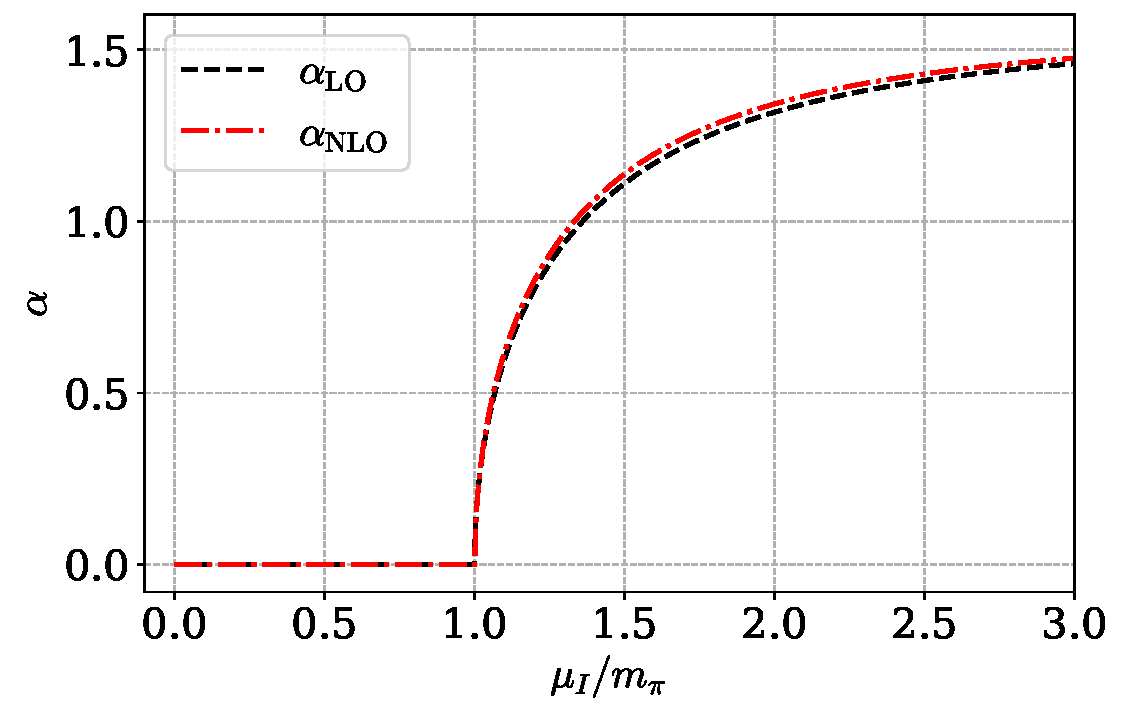
\includegraphics[width=.51\textwidth]{../scripts/figurer/pion_nlo_alpha.pdf}
    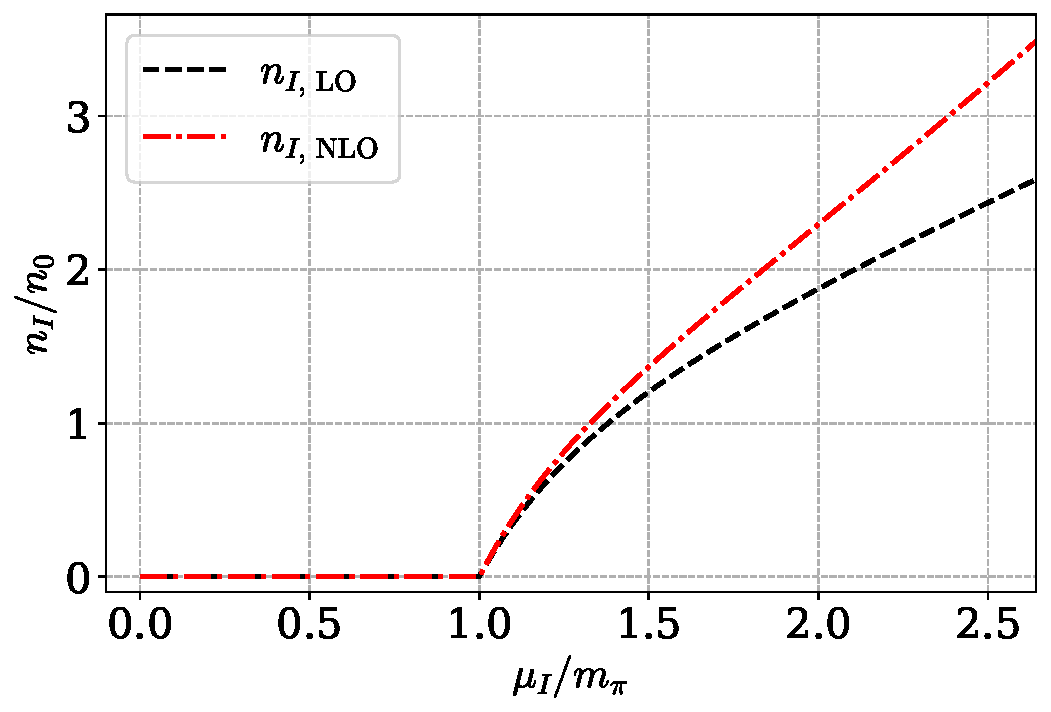
\includegraphics[width=.48\textwidth]{../scripts/figurer/pion_nlo_nI_945.pdf}
    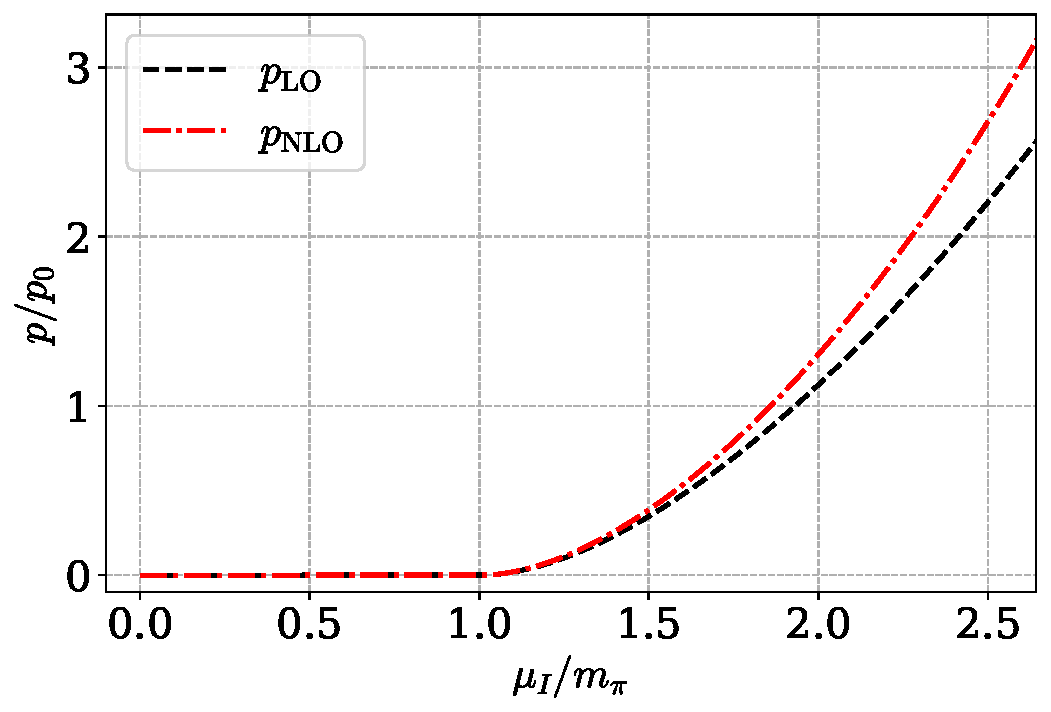
\includegraphics[width=.49\textwidth]{../scripts/figurer/pion_nlo_p_945.pdf}
    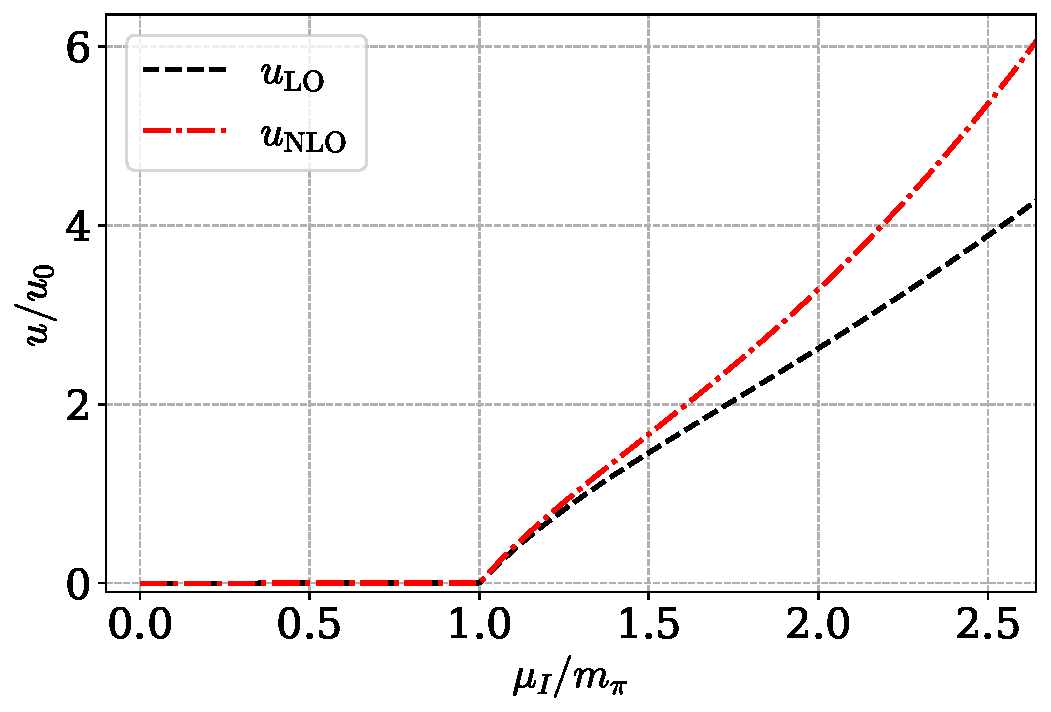
\includegraphics[width=.49\textwidth]{../scripts/figurer/pion_nlo_u_945.pdf}
    \caption{The next-to-leading order results of various thermodynamic quantities, compared to the leading order results. The characteristic quantities are $p_0 = u_0 = m_\pi n_0 = f_\pi^2 m_\pi^2$, and $\mu_I$ is given in units of $m_\pi$.}
    \label{fig: nlo quantitites}
\end{figure}


\begin{figure}
    \centering
    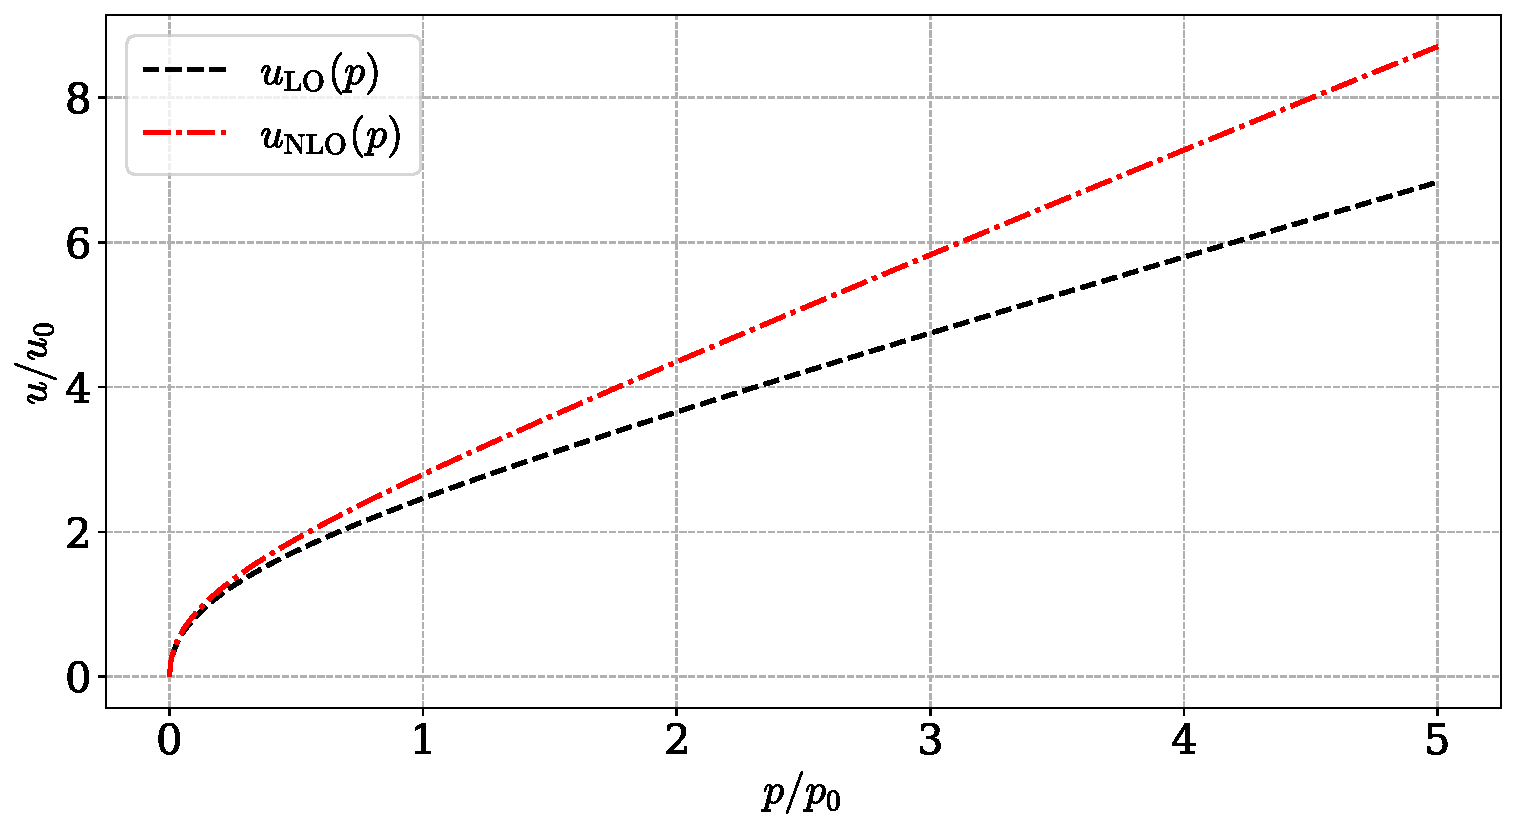
\includegraphics[width=.8\textwidth]{../scripts/figurer/pion_eos_nlo.pdf}
    \caption{The NLO equation of state compared to the LO results. The characteristic quantitites are $u_0 = p_0 = m_\pi^2 f_\pi^2$.}
    \label{fig: nlo eos}
\end{figure}

\begin{figure}[!htb]
    \centering
    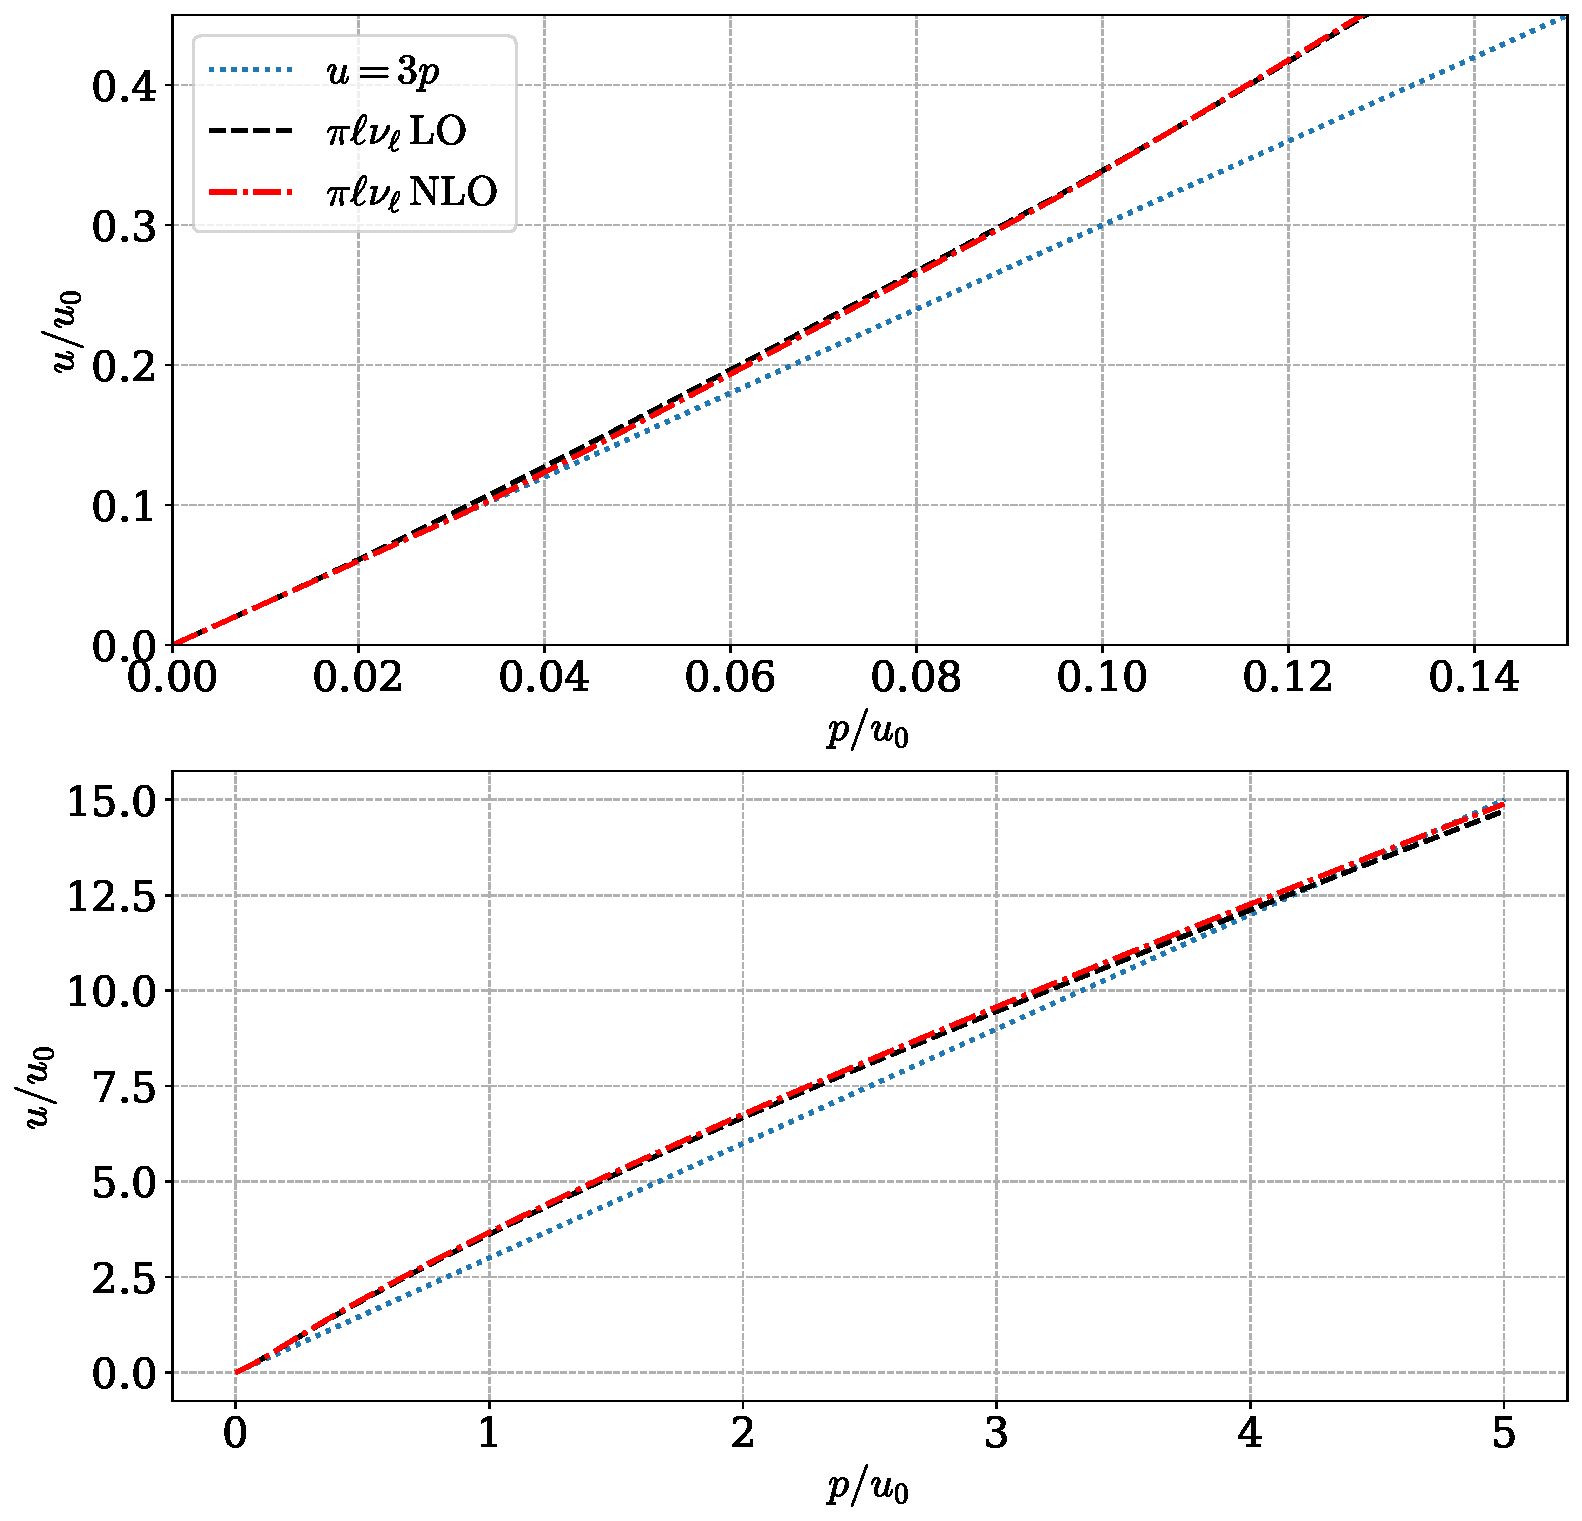
\includegraphics[width=.82\textwidth]{../scripts/figurer/pion_star/neutrino_nlo_eos.pdf}
    \caption{The NLO and LO equation of state for the $\pi \ell \nu_\ell$ system are compared for two different regimes. Energy density and pressure are normalized to their characteristic quantities, $p_0 = u_0 = f_\pi^2m_\pi^2$.}
    \label{fig: eos pi ell nu}
\end{figure}



\begin{figure}[!htb]
    \centering
    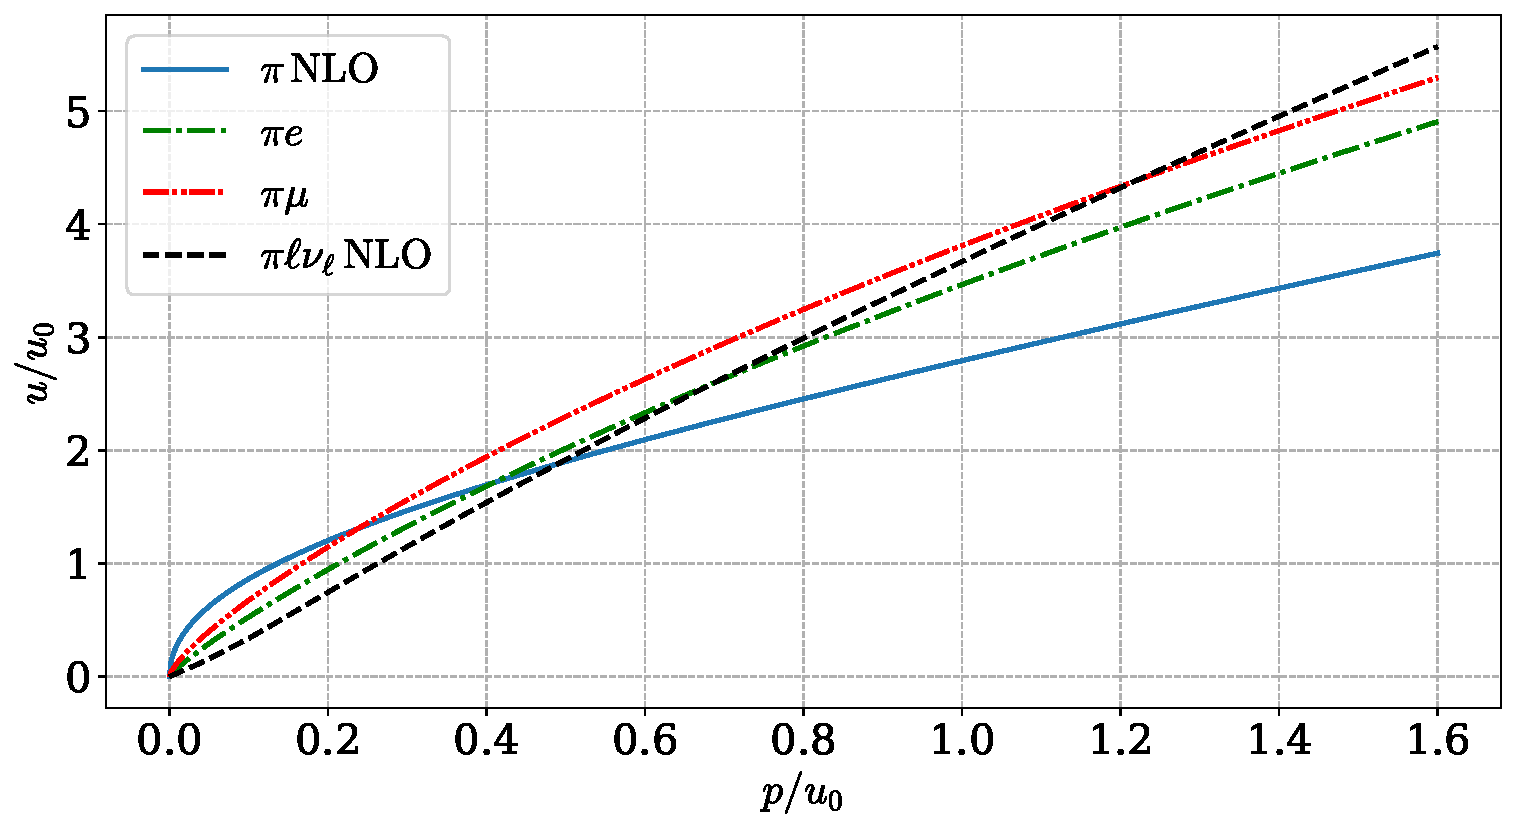
\includegraphics[width=.82\textwidth]{../scripts/figurer/pion_star/pion_all_eos.pdf}
    \caption{
        The equation of state of pion condensate alone, and including other particles.
        Both the pressure and the energy density are normalized to $u_0 = f_\pi^2 m_\pi^2$.
    }
    \label{fig: all eos}
\end{figure}

